\documentclass[12pt,letterpaper]{article}
\usepackage{graphics}
\newcommand{\kg}{\mathrm{kg}}
\newcommand{\m}{\mathrm{m}}
\newcommand{\s}{\mathrm{s}}
\renewcommand{\deg}{\mathrm{deg}}
\newcommand{\cm}{\mathrm{cm}}
\newcommand{\mps}{\m\,\s^{-1}}
\newcommand{\mpss}{\m\,\s^{-2}}
\newcommand{\kgpmmm}{\kg\,\m^{-3}}
\newcommand{\N}{\mathrm{N}}
\newcommand{\J}{\mathrm{J}}
\newcommand{\hp}{\mathrm{hp}}
\newcommand{\Npmm}{\N\,\m^{-2}}
\newcommand{\tv}[1]{\mathbf{\vec{#1}}}
\newcommand{\vvstudent}{\tv{v}_\mathrm{student}}
\newcommand{\vvice}{\tv{v}_\mathrm{ice}}
\newcounter{problem}
\addtolength{\oddsidemargin}{-1in}
\addtolength{\textheight}{\headheight}
\setlength{\headheight}{0in}
\addtolength{\textheight}{\headsep}
\setlength{\headsep}{0in}
\setlength{\marginparwidth}{2in}
\begin{document}

\section*{NYU Physics 1---final exam}

2007 December

\subsection*{Name:}

~ \vfill ~

\clearpage

\paragraph{Problem~\theproblem}\refstepcounter{problem}%
What is the approximate volume $V$ and density $\rho$ of the Earth?
Give some justification for your answers, and give your answers in SI
units.

~ \vfill ~

\paragraph{Problem~\theproblem}\refstepcounter{problem}%
For a good golfer, a $150\,\m$ drive is easy.  As you know from your
famous problem-set problem, you can't ignore air resistance!  But if
you \emph{do} assume that air resistance does not matter, what
velocity (magnitude) $v$ does the ball have at the beginning of its
flight?  Assume that it is hit at $45\,\deg$ to the horizontal.  Show
all your work.

~ \vfill ~

\clearpage

\paragraph{Problem~\theproblem}\refstepcounter{problem}%
In this system of blocks and pulleys, how are the \emph{vector}
accelerations of the two blocks related?  Be sure to be clear about
the directions.%
\marginpar{\includegraphics{../mp/tackle_blocks.eps}}%

~ \vfill ~

\paragraph{Problem~\theproblem}\refstepcounter{problem}%
A golf ball drops from a height of $3\,\m$ onto a concrete floor.
\emph{During the time that the ball is in contact with the floor,}
what is the mean \emph{net} force on the ball?  Assume that the ball
is in contact with the floor for about $10^{-4}\,\s$.  Give your
answer in terms of the gravitational force $m\,g$.

~ \vfill ~

\clearpage

\paragraph{Problem~\theproblem}\refstepcounter{problem}%
A car requires static frictional force $f<\mu\,N$ to maintain traction
in the direction transverse to the direction of motion.  A car travels
on a horizontal, curved path with radius $R$, on a road surface banked
at an angle of $\theta$ to the horizontal, with a coefficient of
static friction $\mu$ between the car and the road.  The car is
traveling at the maximum possible speed that friction allows.  The net
force $F$ acting on the car can be drawn with arrows as a vector sum
of the individual vector forces acting on the car.  Draw this vector
sum.  Make sure your diagram is not at all ambiguous about what angles
are $\theta$, what angles are right angles, and which way is
horizontal and which way is vertical.

~ \vfill ~

\paragraph{Problem~\theproblem}\refstepcounter{problem}%
Derive Kepler's third law (that relating period to radius) for
circular orbits from the gravitational force law $F=G\,M\,m/r^2$.  You
may use dimensional arguments if you wish.

~ \vfill ~

\clearpage

\paragraph{Problem~\theproblem}\refstepcounter{problem}%
A rod of mass $m$ and length $\ell$ is attached to a wall with a
frictionless pivot and also to a cable making an angle $\theta$ to the
horizontal.  The cable holds the rod up against gravity as shown.
What is the tension in the cable?  Show all your work.%
\marginpar{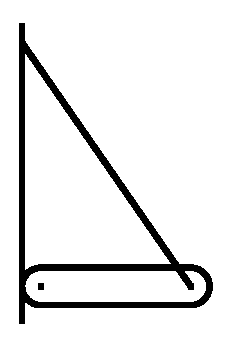
\includegraphics{../eps/horizontal_rod.eps}}%

~ \vfill ~

\paragraph{Problem~\theproblem}\refstepcounter{problem}%
A small bullet of mass $m$ traveling at speed $v$ lodges in the end of
a stick of mass $m$ and length $\ell$ as shown.  What is the final
rotational speed $\omega$ of the bullet+stick system?  Recall that the
moment of inertia of a thin stick of length $\ell$ around its center
of mass is $(1/12)\,m\,\ell^2$ and treat the bullet as a point
particle for the purposes of moment of inertia calculations.  Show all
your work.%
\marginpar{\includegraphics{../mp/bullet_stick.eps}}%

~ \vfill ~

\clearpage

\paragraph{Problem~\theproblem}\refstepcounter{problem}%
In a problem set I asked you to numerically integrate the acceleration
of a car putting out a constant power of $130\,\hp$.  I started the
integration when the car was traveling at $5\,\mps$ not $0\,\mps$.
Why did I do this?

~ \vfill ~

\paragraph{Problem~\theproblem}\refstepcounter{problem}%
Explain why the astronauts in the Space Shuttle are weightless.

~ \vfill ~

\clearpage

~ \vfill ~

This page intentionally left blank.

~ \vfill ~

\end{document}
